\newpage
\section{Spins, Qubits and Linear Operators}

In the quantum world, state and measurement are two different things.

\subsection{The Stern-Gerlach Experiment}
In the Stern-Gerlach experiment, a narrow beam of silver atoms passes through an electromagnet [with a nonuniform $\vec{B}(z)=B(z)\hat{z}$] and then lands on a glass detector plate.

\begin{figure}[H]
    \centering
    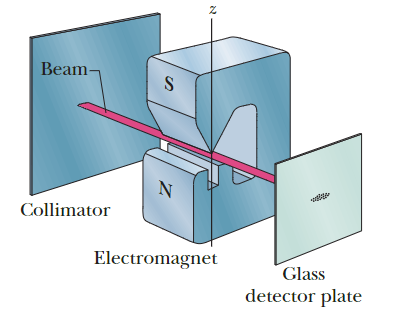
\includegraphics[width=0.309\textwidth]{QI3/The Stern-Gerlach Experiment}
    \caption{The Stern-Gerlach Experiment}
\end{figure}

In fact, spin states also belong to the 2D complex vector space $\mathbb{C}^2$. 

\subsection{Spin, Qubit, and the Bloch Sphere}
The isolated quantum spin $(S = 1/2)$ is our second realization of the general class of two-level systems which we call \hl{qubits}, or quantum bits.

A classical computer operates on strings of zeros and ones, such as 1001001001. Each position in such a string is called a (classical) bit, and it contains either a 0 or a 1. The abstract bit can be represented by a physical system. 

We can take the two states of a classical bit to be represented by two orthogonal unit vectors in a two-dimensional space,
\begin{align*}
    \ket{0}\equiv \ket{\uparrow}=\begin{pmatrix}
        1\\ 0
    \end{pmatrix}, \,
    \ket{1}\equiv \ket{\downarrow}= \begin{pmatrix}
        0\\ 1
    \end{pmatrix}
\end{align*}
Classically, we either have state $\ket{0}$, or state $\ket{1}$, but not both simultaneously.

In quantum mechanics, however, the two states can be superimposed, i.e., we promote the states of a classical bit to be two basis vectors in $\mathbb{C}^2$.

As we know, a general state of a qubit is
\begin{align*}
    \ket{\phi}=\alpha\ket{0}+\beta\ket{1}=\begin{pmatrix}
        \alpha \\ \beta
    \end{pmatrix}, \, \alpha, \beta\in \mathbb{C}
\end{align*}
normalized by (the probabilistic interpretation)
\begin{align*}
    \braket{\phi | \phi }=|\alpha|^2+|\beta|^2=1
\end{align*}

We can parametrize it, alternatively, by
\begin{align*}
    \ket{\phi}=\cos\frac{\theta}{2}\ket{0}+e^{i\phi}\sin\frac{\theta}{2}\ket{1}
\end{align*}
and represented it by a point on the \hl{Bloch sphere}.

\begin{figure}[H]
    \centering
    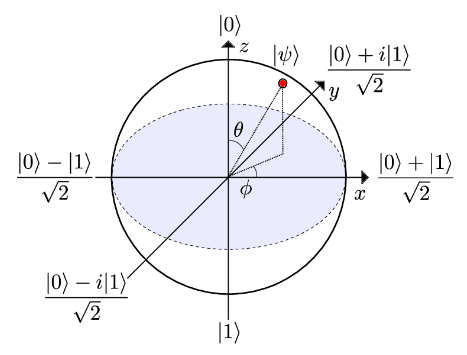
\includegraphics[width=0.309\textwidth]{QI3/A spin state}
    \caption{The Bloch sphere}
\end{figure}

\subsection{Linear Operators and Matrices}

\subsubsection{Measuring a Quantum Spin}

Knowing a quantum state, on the other hand, means knowing as much as can be known about how the system was prepared. Perhaps the most difficult things to accept is that quantum mechanics is unavoidably unpredictable. It is a complete calculus of probabilities.

At the center of the calculus is the idea of an observable or a measurable, i.e., a property one can measure with a proper apparatus. 

\subsubsection{Linear Operators}
We will introduce an axiom: physical observables are described by linear operators.

A map $M: \mathbb{C}^n \rightarrow \mathbb{C}^n$ is a \hl{linear operator} if 
\begin{align*}
    M(\mu\ket{x}+\nu\ket{y})=\mu M\ket{x}+ \nu M\ket{y}
\end{align*}
is satisfied for arbitrary $\ket{x}, \ket{y}\in \mathbb{C}^n$ and $\mu, \nu \in \mathbb{C}$. 

The definition expresses the following facts. 
\begin{enumerate}
    \item M acts on a vector $\ket{a}$ to given $\ket{b}$ in the same space of states:
    \begin{align*}
        M\ket{a}=\ket{b}
    \end{align*}
    \item When M acts on a multiple of an input vector, it gives the same multiple of the output vector:
    \begin{align*}
        M\zeta \ket{a} = \zeta\ket{b}.
    \end{align*}
    \item When M acts on a sum of vectors, the results are simply the sum of the output vectors:
    \begin{align*}
        M\{\ket{a} + \ket{b}\} = M\ket{a} + M\ket{b}.
    \end{align*}
\end{enumerate}

\subsubsection[Matrix Representation]{Matrix Representation of Linear Operators}

Given the choice of basis vectors, bra and ket vectors are represented by row and column vectors. If the vector space is N-dimensional, we can choose a set of N orthonormal ket-vectors $\ket{j}$ and their dual bra-vectors $\bra{j}$. 

In component form, we can write
\begin{align*}
    \ket{a}=\sum_{j=1}^N \alpha_j\ket{j}, \, \ket{b}=\sum_{j=1}^N \beta_j \ket{j}
\end{align*}

Plugging the substitutions into $M\ket{a} = \ket{b}$, we obtain
\begin{align*}
    \sum_{j=1}^N M\ket{j}\alpha_j=\sum_{j=1}^N\beta\ket{j}
\end{align*}

The inner product of both sides with a particular basis vector $\bra{k}$ gives
\begin{align*}
    \sum_{j=1}^N \braket{k|M|j}\alpha_j=\sum_{j=1}^N\beta_j \braket{k|j}=\beta_k
\end{align*}
where the second identity is obtained because $\braket{k|j}=\delta_{kj}$. 

Symbolically, we can define an $N\times N$ matrix
\begin{align*}
    M=\begin{pmatrix}
        m_{11} & m_{12} & \cdots & m_{1N} \\
        m_{21} & m_{22} & \cdots & m_{2N} \\
        \vdots & \vdots & \ddots & \vdots \\
        m_{N1} & m_{N2} & \cdots & m_{NN} \\
    \end{pmatrix}
\end{align*}
where $m_{kj}\equiv \braket{k|M|j}$ are called matrix elements.

The inner product of $M\ket{a}=\ket{b}$ with $\bra{k}$ becomes
\begin{align*}
    \sum_j m_{kj}\alpha_j=\beta_k
\end{align*}
for $k=1,2,\dots,N$. 

One recognizes that this is nothing but the matrix multiplication
\begin{align*}
    \begin{pmatrix}
        m_{11} & m_{12} & \cdots & m_{1N} \\
        m_{21} & m_{22} & \cdots & m_{2N} \\
        \vdots & \vdots & \ddots & \vdots \\
        m_{N1} & m_{N2} & \cdots & m_{NN} \\
    \end{pmatrix}\begin{pmatrix}
        \alpha_1 \\ \alpha_2 \\ \vdots \\ \alpha_N
    \end{pmatrix}=\begin{pmatrix}
        \beta_1 \\ \beta_2 \\ \vdots \\ \beta_N
    \end{pmatrix}
\end{align*}
which can simply be abbreviated as $M\ket{a}=\ket{b}$, in which $M$, $\ket{a}$, $\ket{b}$ are now represented by the matrix and two vectors.

\subsubsection{Eigenvalues and Eigenvectors}
For the application of a linear operator on a vector, such as
$M\ket{a}=\ket{b}$, we do not expect, in general, $\ket{b}=\alpha\ket{a}$,
where $\alpha\in \mathbb{C}$.

However, along certain directions, we find ket-vectors $\ket{\lambda}$such that
\begin{align*}
    M\ket{\lambda} = \lambda\ket{\lambda},
\end{align*}
where $\lambda$ are called \hl{eigenvalues}, while $\ket{\lambda}$ the corresponding \hl{eigenvectors}.

In general, eigenvalues are complex numbers. For example,
\begin{align*}
    \begin{pmatrix}
        0 & -1 \\ 1 & 0 
    \end{pmatrix}\begin{pmatrix}
        1\\ i
    \end{pmatrix}=-i\begin{pmatrix}
        1\\ i
    \end{pmatrix}
\end{align*}

However, observable quantities in quantum mechanics are represented by Hermitian operators, i.e., linear operators that are equal to their own Hermitian conjugate ($M^{\dagger}=\overline{\left[M^T\right]}$, 转置复共轭). 
\begin{itemize}
    \item If $M\ket{a}=\ket{b}$, then $\bra{a}M^{\dagger}=\bra{b}$ in general. For Hermitian $M$, we further have $\bra{a}M=\bra{b}$. 
    \item It follows that the eigenvalues of a Hermitian matrix are real.
\end{itemize}

According to mathematics, the eigenvectors of a Hermitian operator form an orthonormal basis–this serves as a foundation of quantum mechanics. 
\begin{itemize}
    \item The eigenvectors of a Hermitian operator are a complete set, i.e. any vector the operator can generate can be expanded as a sum of its eigenvectors.
    \item If $\lambda_1$ and $\lambda_2$ are two unequal eigenvalues of a Hermitian operator, then the corresponding eigenvectors are orthogonal.
    \item Even if the two eigenvalues are equal (i.e., degenerate), the corresponding eigenvectors can be chosen to be orthogonal. 
\end{itemize}

Therefore, we often replace an operator by its spectral decomposition (note we insert two identity operators)
\begin{align*}
    M=\sum_{\lambda \lambda'}\ket{\lambda}\braket{\lambda|M|\lambda'}\bra{\lambda'}=\sum_{\lambda}\lambda\ket{\lambda}\bra{\lambda}=\sum_{\lambda}\lambda P_{\lambda}
\end{align*}

\subsection{The \textbf{Principles }of Quantum Mechanics}
States of a system are represented by vectors in a complex vector space.
\begin{enumerate}
    \item The observables or measurable quantities of \\quantum mechanics are represented by linear operators $L$.
    \item The possible results of a measurement are the eigenvalues $\lambda$ of the operator that represents the observable.
    \item Unambiguously distinguishable states are represented by orthogonal vectors.
    \item If $\ket{\phi}$ is a state-vector, and the observable $L$ is measured, the probability to observe $\lambda$ is $P_{\lambda} = \braket{\phi | \lambda}\braket{\lambda|\phi}$, where $\ket{\lambda}$ is the corresponding eigenvector.
\end{enumerate}

\subsubsection{Constructing Spin Operators}
\textbf{Principle 1} states that each component of spin (denoted by $\sigma$) is represented by a linear operator. We begin with $\sigma_z$ along the $z$ direction.

\textbf{Principle 2} states that $\sigma_z$ has two eigenvalues $\pm 1$ with
corresponding eigenvectors, i.e.,
\begin{align*}
    \sigma_z\ket{0}=\ket{0},\, \sigma_z\ket{1}=-\ket{1}
\end{align*}

\textbf{Principle 3} emphasizes that $\braket{0|1} = 0$. Therefore, as we learned above, the matrix representation of $\sigma_z$ is
\begin{align*}
    \sigma_z=\begin{pmatrix}
        \braket{0|\sigma_z|0} & \braket{0|\sigma_z|1}\\
        \braket{1|\sigma_z|0} & \braket{1|\sigma_z|1}
    \end{pmatrix}=\begin{pmatrix}
        1 & 0\\ 0 & -1
    \end{pmatrix}
\end{align*}
where we also use $\braket{0|0} =\braket{1|1} = 1$.

\textbf{Principle 4} states that for a spin in $ \ket{\phi}=\alpha\ket{0}+\beta\ket{1}$, $|\alpha|^2=\alpha*\alpha$ is the probability of the spin being up, or that the spin would be measured as $\sigma_z = +1$. Likewise, $|\beta|^2=\beta*\beta$ is the probability of the spin being down, or that the spin would be measured as $\sigma_z = -1$.

To construct $\sigma_x$ and $\sigma_y$, 

We can also rotate the apparatus to align along x axis and measure the spin component to be either +1 or -1. This means that we can define two basis states by
\begin{align*}
    \sigma_x\ket{r}=\ket{r}, \, \sigma_x\ket{l}=-\ket{l}
\end{align*}
Thus, we need to know, e.g., what $\alpha$ and $\beta$ are, such that
\begin{align*}
    \ket{r}=\alpha\ket{0}+\beta\ket{1}
\end{align*}
In physics, we determine them by experimental measurements, not mathematical axioms.

Therefore, experiments tell us that
\begin{align*}
    \ket{r}=\frac{1}{\sqrt{2}}\ket{0}+\frac{e^{i\phi}}{\sqrt{2}}\ket{1}
\end{align*}

There is some ambiguity in choosing the phase $\phi$, but it is nothing more than the ambiguity in our choice of the exact direction for the x axis. We can simply choose $\phi = 0$, so
\begin{align*}
    \ket{r}=\frac{1}{\sqrt{2}}\ket{0}+\frac{1}{\sqrt{2}}\ket{1}
\end{align*}
Using $\braket{r|l}=0$ and $\braket{l|l}=1$, we find
\begin{align*}
    \ket{l}=\frac{1}{\sqrt{2}}\ket{0}-\frac{1}{\sqrt{2}}\ket{1}
\end{align*}
There can be an overall phase factor in $\ket{r}$ and $\ket{l}$, but it is not measurable. 

The matrix representation of $\sigma_x$ must, then, satisfy
\begin{align*}
    \begin{pmatrix}
        (\sigma_x)_{00} & (\sigma_x)_{01}\\ (\sigma_x)_{10} & (\sigma_x)_{11}
    \end{pmatrix}\begin{pmatrix}
        \frac{1}{\sqrt{2}} \\ \frac{1}{\sqrt{2}}
    \end{pmatrix}=&\begin{pmatrix}
        \frac{1}{\sqrt{2}} \\ \frac{1}{\sqrt{2}}
    \end{pmatrix} \\
    \begin{pmatrix}
        (\sigma_x)_{00} & (\sigma_x)_{01}\\ (\sigma_x)_{10} & (\sigma_x)_{11}
    \end{pmatrix}\begin{pmatrix}
        \frac{1}{\sqrt{2}} \\ -\frac{1}{\sqrt{2}}
    \end{pmatrix}=&-\begin{pmatrix}
        \frac{1}{\sqrt{2}} \\ -\frac{1}{\sqrt{2}}
    \end{pmatrix} 
\end{align*}

The solution to the two matrix equations is
\begin{align*}
    \sigma_x=\begin{pmatrix}
        0 & 1\\1 &0
    \end{pmatrix}
\end{align*}

In a similar, but more complicated way, we can obtain
\begin{align*}
    \sigma_y=\begin{pmatrix}
        0 & -i \\ i & 0
    \end{pmatrix}
\end{align*}
whose eigenvectors, with eigenvalues $\pm 1$, are
\begin{align*}
    \ket{i}=\frac{1}{\sqrt{2}}\ket{0}+\frac{i}{\sqrt{2}}\ket{1}, \, \ket{o}=\frac{1}{\sqrt{2}}\ket{0}-\frac{i}{\sqrt{2}}\ket{1}
\end{align*}

\subsubsection{Along an Arbitrary Direction}
The three spin operators, represented by
\begin{align*}
    \sigma_x=\begin{pmatrix}
        0 & 1\\1 &0
    \end{pmatrix}, \, 
    \sigma_y=\begin{pmatrix}
        0 & -i \\ i & 0
    \end{pmatrix}, \, 
    \sigma_z=\begin{pmatrix}
        1 & 0 \\ 0 & -1
    \end{pmatrix}
\end{align*}
are known as \hl{Pauli matrices}.
It is tempting to write
\begin{align*}
    \vec{\sigma}=\sigma_x \hat{x}+ \sigma_y \hat{y} + \sigma_z \hat{z}
\end{align*}
This is correct. In fact, spin is a 3-vector operator.


It is good time to distinguish the two notions of vectors.
\begin{itemize}
    \item We live in a 3D world. Spin, like displacement and momentum,
    is a 3-vector. It has operator (not scalar) components along the
    three spatial directions.
    \item The quantum state of a spin is a state-vector in a 2D complex
    vector spaces (of spin states). 
\end{itemize}

Therefore, the relevant operator for measuring the spin along an arbitrary direction $\hat{n} = (n_x , n_y , n_z )$ is 
\begin{align*}
    \sigma_n&=\vec{\sigma}\cdot \hat{n}=\sigma_x n_x+ \sigma_y n_y + \sigma_z n_z\\
    &=\begin{pmatrix}
        n_z & n_x-in_y \\ n_x+in_y & -n_z
    \end{pmatrix}
\end{align*}
One can check that the eigenvalues, or the measurement results, are, again, $\pm 1$.

\begin{align*}
    \sigma_z=\ket{0}\bra{0}-\ket{1}\bra{1}
\end{align*}

\subsubsection{Irreversibility of Measurement}
Measurement is like blocking one of the paths. Along the other path, you either get the particle, or you do not. You do not know when you get it, but you know the probability of getting it.

Quantum measurement is an irreversible operation. After the measurement, the system is in one of the eigenstates. The pre-measurement state collapses or reduces to the post-measurement state, as a consequence of the measurement (the Copenhagen interpretation). 

We emphasize that when an operator acts on a state-vector, it produces a new state-vector in general. The new vector has nothing to do with the post-measurement state, although we can use it to calculate the average or expectation value of the measurable quantit (退相干丢失了信息). 

L. Susskind and A. Friedman, Quantum Mechanics (Basic Books, 2014), Chaps. 3-4.